\subsection{Point of sail}
A sailboat can achieve velocity by catching the wind in the sail at different angles. This is called point of sail and the velocity is dependent on the dinghies displacement from the true wind direction, the wind experienced for a stationary object, where the velocity is a resultant of the force vector created by the wind depending on the alignment of the sail and the direction from the wind direction. There are five different states of point of sail that are divided into degrees away from the true wind origin. These are
\begin{labeling}{alligator}
\item [Luffing] (no propulsive force) angle between 0-30\degree
\item [Close-hauled] (lift) angle between 30-50\degree
\item [Beam reach] (lift) angle 90\degree
\item [Broad reach] (lift–drag) angle aound 135\degree
\item [Running] (drag) angle around 180\degree
\end{labeling}
and are represented in Fig. \ref{points-sail}. A sailor wants to prevent the sail from luffing, luffing is when the sail starts to flap in the wind and no propulsive force is achieved. When the dinghy is in the close-hauled and beam reach state the sail produces lift force that is produced from the average pressure differences on the windward and leeward side of the sail where the pressure is higher on the windward surface thus acting like a wing propelling the dinghy. When the dinghy is in the broad reach state both lift and also drag propels the dinghy. Drag acts like a parachute that that catches the wind and propels the dinghy. The sideway force induced on the boat also introduces drift perpendicular to the relative bearing. This is counteracted by lowering a centerboard which also counteracts the dinghy from heeling.
\begin{figure}[H]
\centering
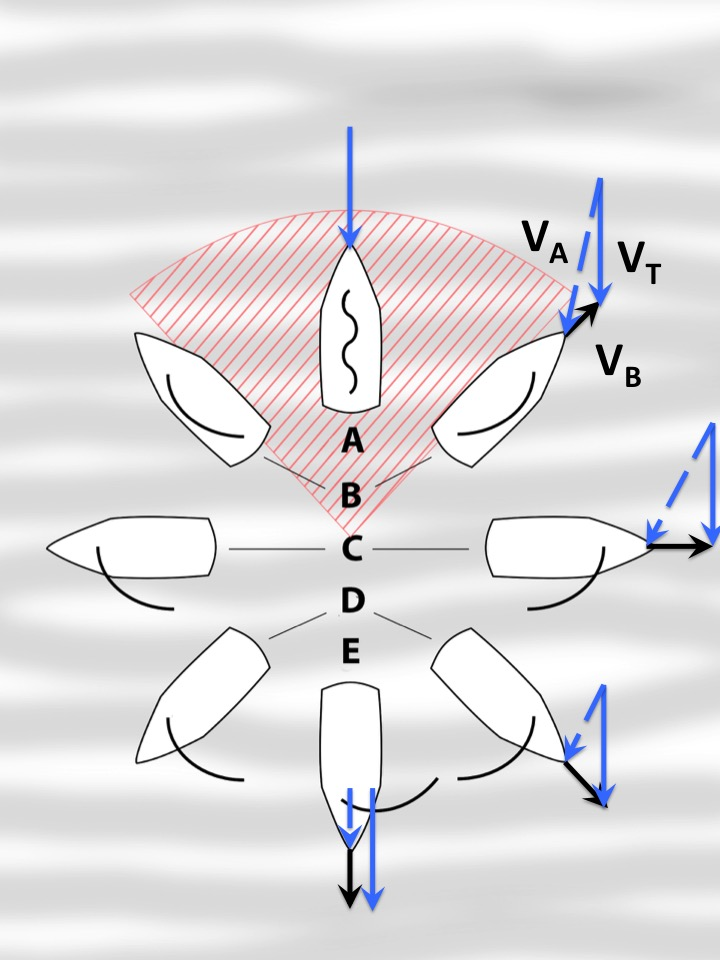
\includegraphics[width=0.6\textwidth]{Figures/Points_of_sail.jpg}
\caption{Points of sail}
\label{points-sail}
\end{figure}
\begin{figure}[H]
\centering
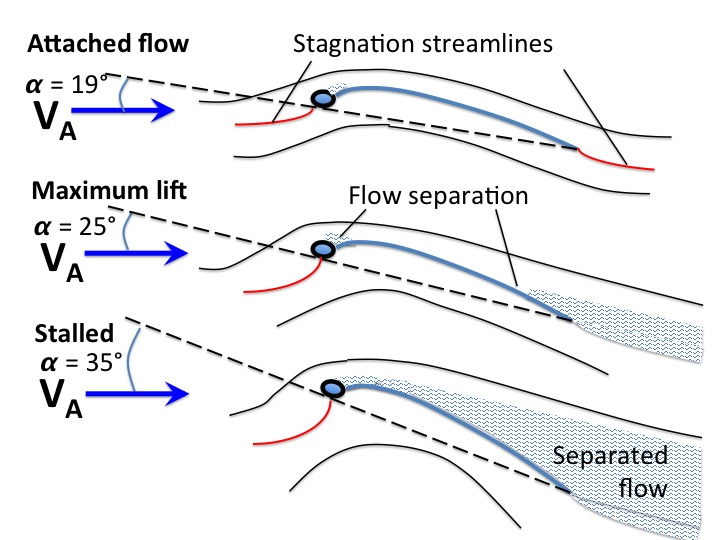
\includegraphics[width=0.6\textwidth]{Figures/max_lift.jpg}
\caption{Sail angles of attack}
\label{max_liftl}
\end{figure}
\subsection{Velocity}
The main goal in sailing is to maximize the efficiency at which the forces on the sail translates into the velocity of the dinghy. A layman might expect that the fastest velocity is achieved when the dinghy is parallel to the true wind, however, this is not true. The apparent wind which is the wind experienced from the dingy perspective is what propels the dingy. When sailing parallel to the wind the dinghies speed can never exceed the speed of the wind\cite{sail-force}. By sailing upwind close-hauled the apparent wind is increased as the dingy accelerates until the drag from the water exceeds the forward force created by the wind. To further increase the velocity of the dingy should not be heeling excessively. This is to prevent the centerboard from acting as a rudder and changing the bearing, introducing more drag from the stern rudder when compensating for the bearing changes. As mentioned earlier the centerboard helps to counteract heeling but also the sailor can prevent this by hiking, leaning outside of the hull to alter the center of mass for the dinghy. Lastly when all other measures were taken the sailor must perform reefing and reducing the area of the sail and lowering the center of effort from the sails.
